\chapter*{Behavioural Experiment}
\addcontentsline{toc}{chapter}{Behavioural}
%In order to investigate whether the deep learning neural net was identifying characteristics of the music that humans can consciously identify we ran a followup behavioural experiment. 
\subsection*{Participants}
9 participants (4 male), aged 22-28, with normal hearing and no history of head injuries took part in this study. Six participants had formal music training (2-15 years), and four of the participants played instruments regularly at the time of data collection. On average participants listened attentively to music 1.5 hours per day and had music playing in the background for 3.6 hours per day. 
\subsection*{Procedure}
The 12 stimuli used were the same songs as those used in the original experiment (See \autoref{tab:stimuli_information}.)
The experiment had two parts and lasted about 50 mins.
First, participants listened to each of the 12 stimuli and pressed a button when (and if) they recognized the piece of music.
The timing of their key press was recorded. 
During the second part of the experiment participants were presented with all possible paired combinations of stimuli (78 pairs). 
They listened to the first song followed immediately by the second and then rated how similar they felt the two songs sounded on a scale from 0-100 (0=the songs sound nothing alike, 100=the songs sound exactly the same).
Participants were asked to focus on how generally similar the two songs sounded and not to worry about being correct.

\subsection*{Results}
In order to determine whether the periods of time highlighted by the neural net in layer 3 of \autoref{fig:model_W} are representative of a moment of recognition we collected the average time at which people recognize these musical pieces (\autoref{fig:RecognitionTime}). 
From these results it does not look like the highlighted time periods from layer 3 of the neural net are related to the moment at which people recognize the piece of music. 

\begin{figure}[h] 
  \begin{center}
%    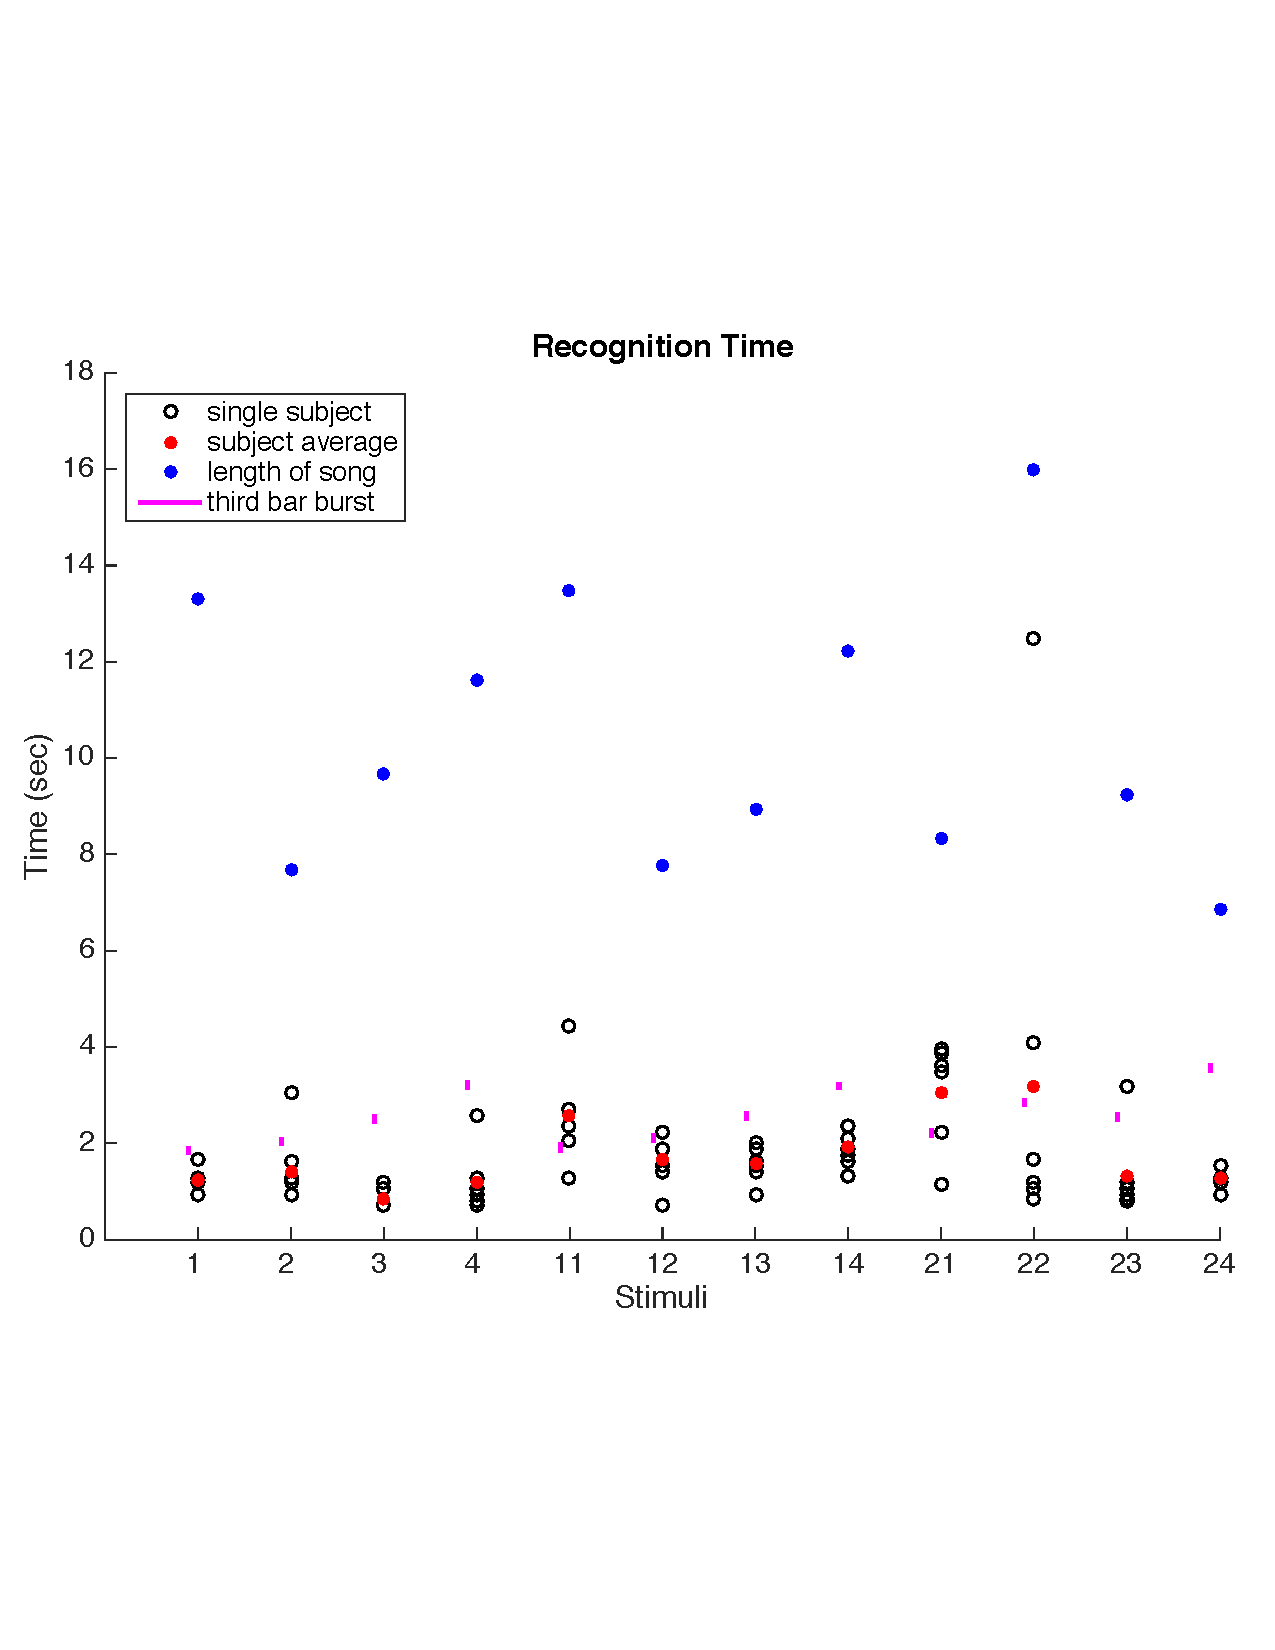
\includegraphics[width=\textwidth,keepaspectratio=true]{Figures/RecognitionTimeGraph}
        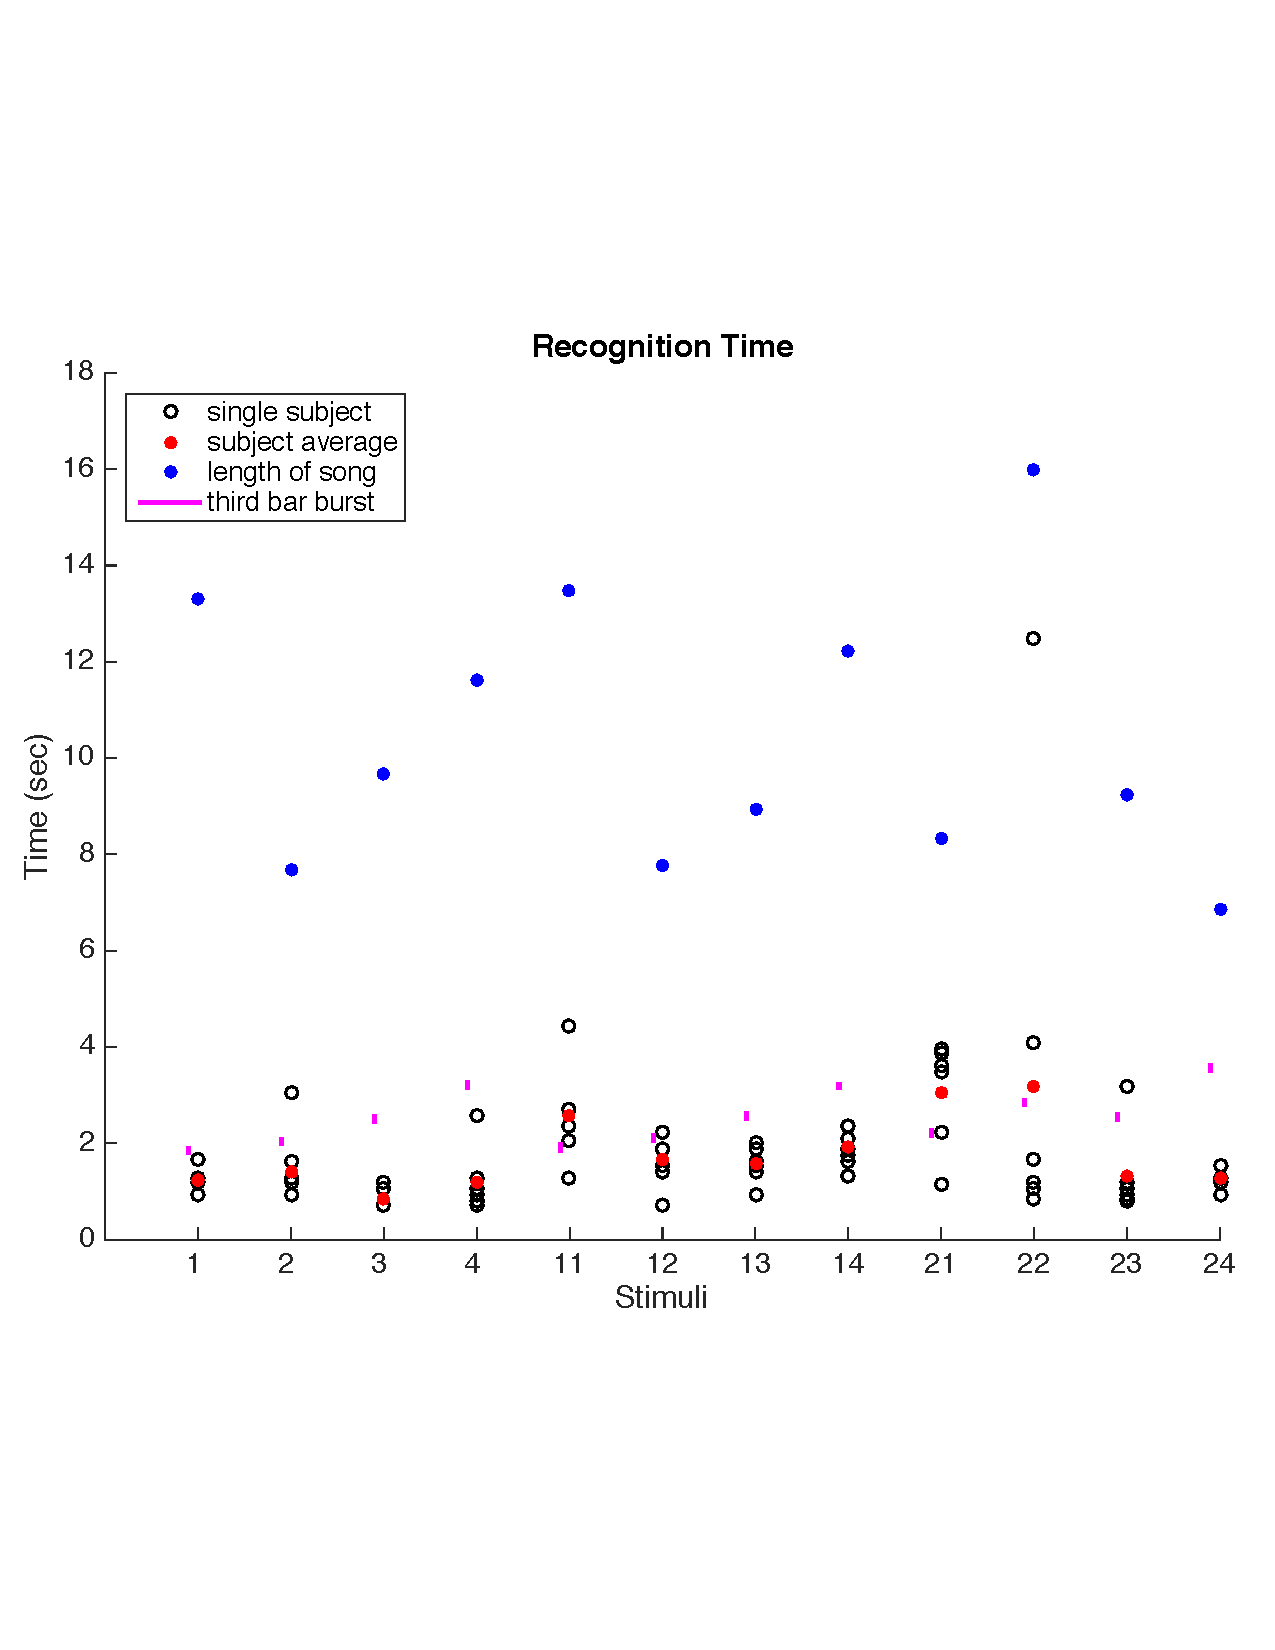
\includegraphics[scale=0.7]{Figures/RecognitionTimeGraph}
%   \\\vspace{-0.8em}
    \caption{Average time it takes for participants to recognize these stimuli (red). Individual data is shown in black and song length is shown in blue. The magenta bars indicate the highlighted time periods from layer three in the neural net (\autoref{fig:model_W_confusion}).}
    \label{fig:RecognitionTime}
  \end{center}
%  \vspace{-1em}
\end{figure}

The second part of the experiment asked participants to give similarity ratings of pairs of songs in order to determine whether the neural net confuses songs that humans rate as similar. 
\autoref{fig:Similarity} shows the similarity rating results. 
As expected, participants are close to perfect at identifying identical songs. 
Lyric/non-lyric pairs of songs were also rated as highly similar and that is seen in the four, dark squares parallel to the diagonal.

The values seen in \autoref{fig:model_W_binary_confusion} can be interpreted as ``dissimilarity'' scores, so we took their inverse (100 - score) to produce similarity scores and correlated this matrix with the average similarity ratings given by our participants.
A correlation of r=0.0012 was calculated (p$>$0.05).
This lack of correlation indicates that the neural net is doing something different than humans when determining similarities between stimuli. 

\begin{figure}[h] 
  \begin{center}
%    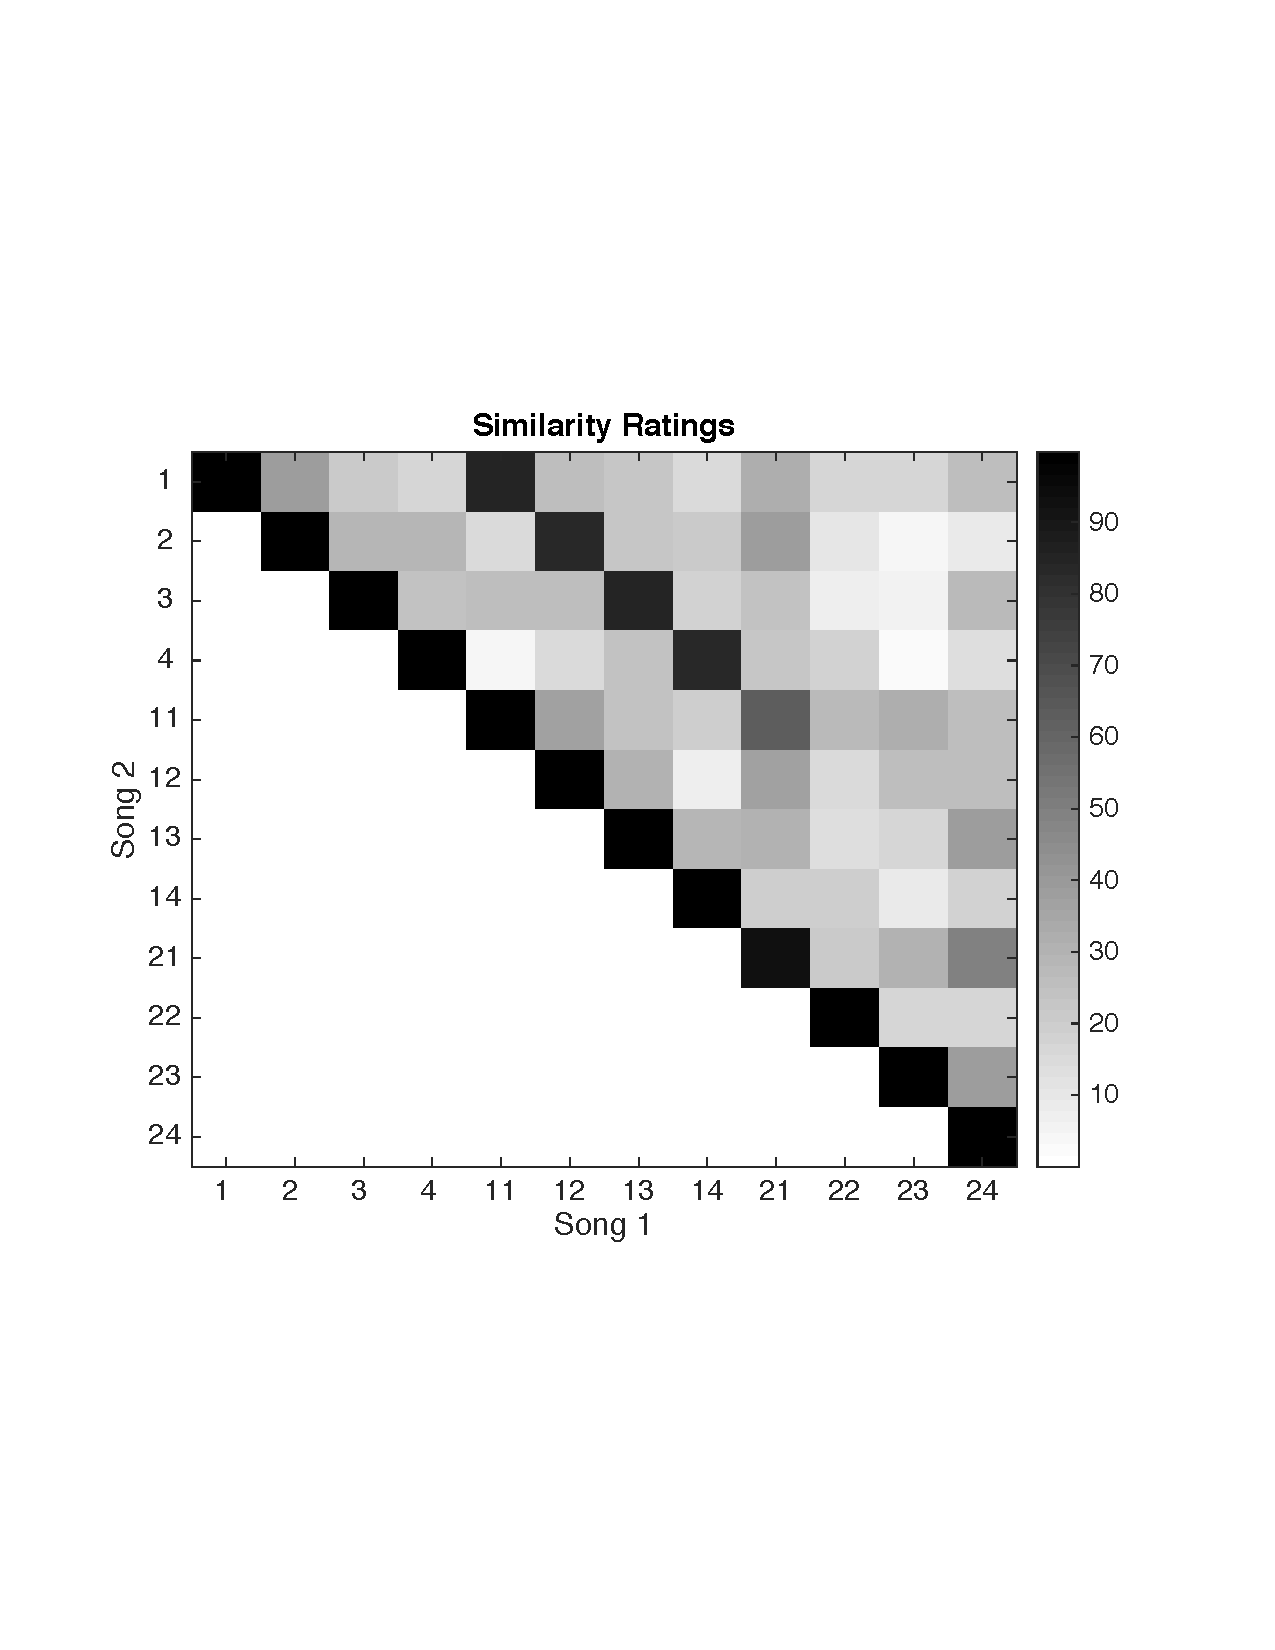
\includegraphics[width=\textwidth,keepaspectratio=true]{Figures/Similarity}
    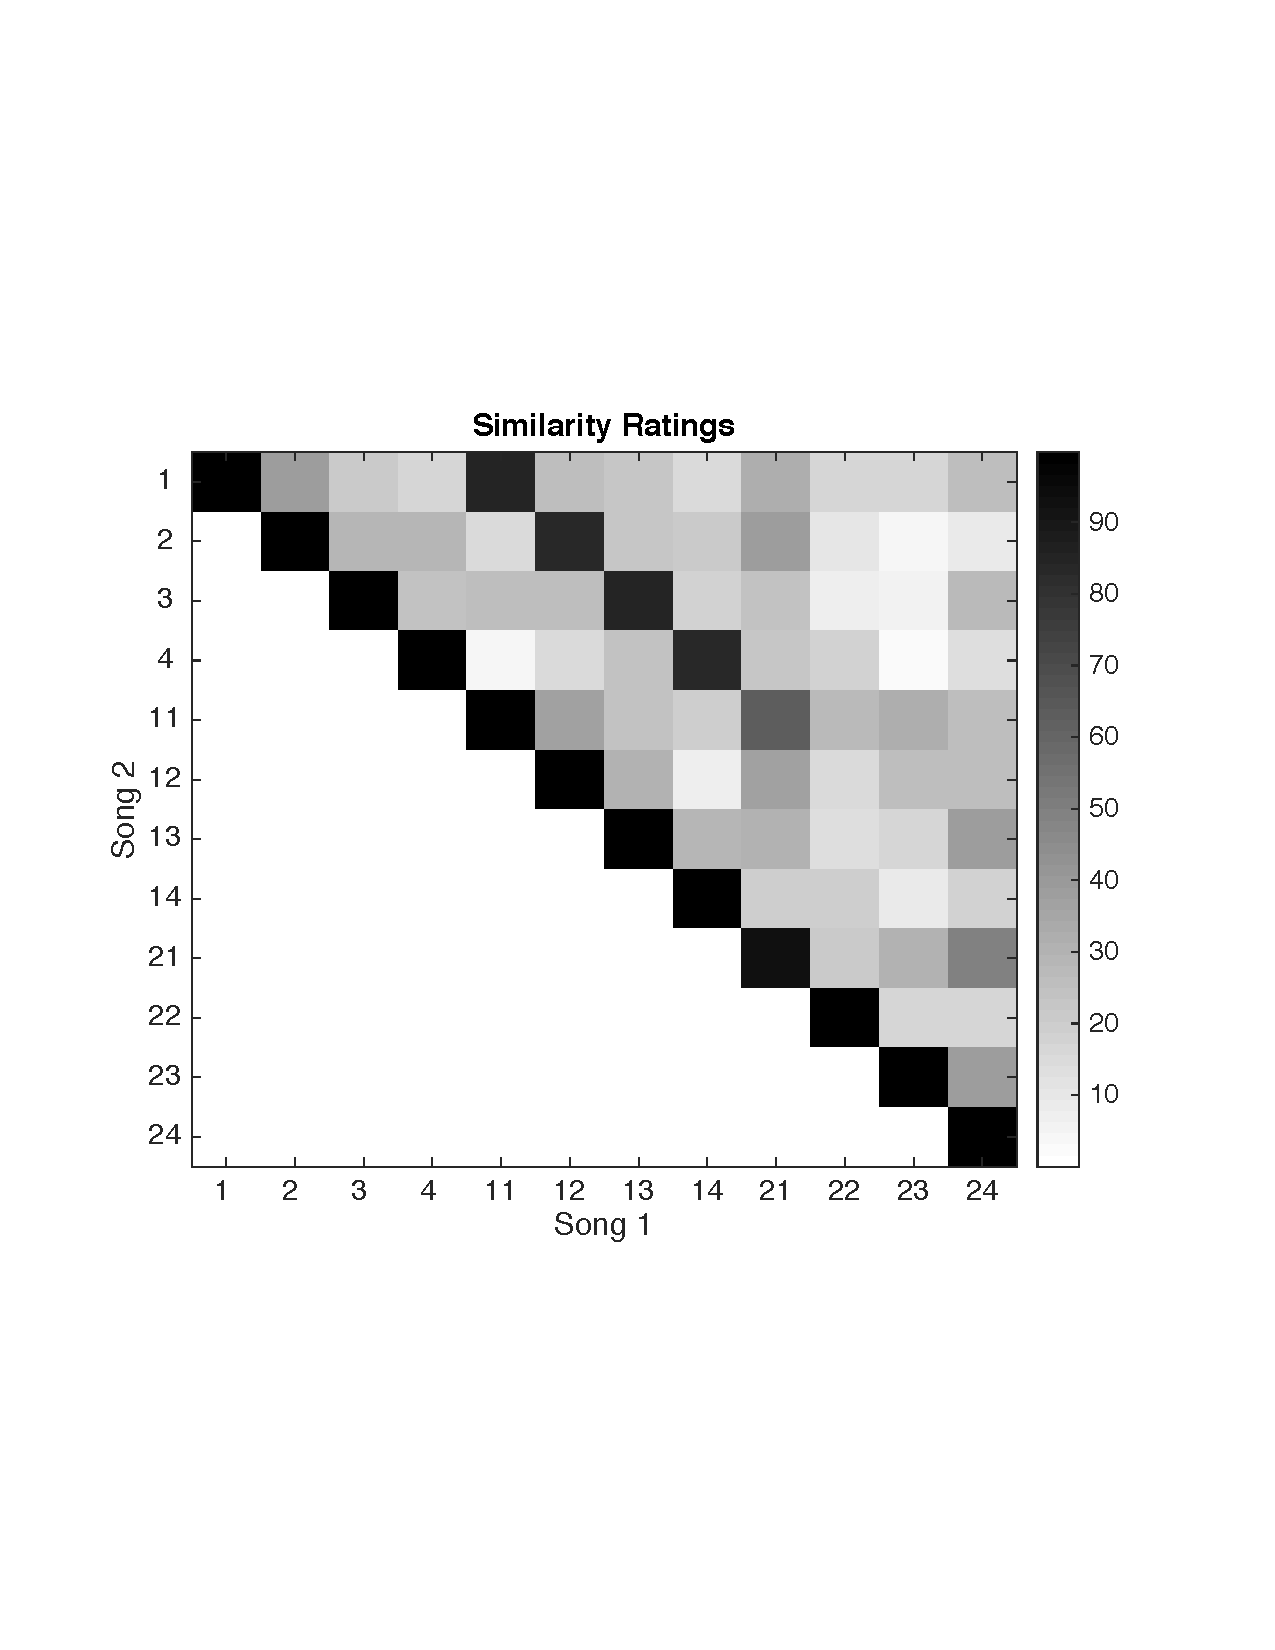
\includegraphics[scale=0.6]{Figures/Similarity}
%   \\\vspace{-0.8em}
    \caption{Similarity ratings (from 0-100) of binary comparisons of all stimuli.}
    \label{fig:Similarity}
  \end{center}
%  \vspace{-1em}
\end{figure}
